% =====================================================================
% Slide 12: Stage 5b -- NN-driven MEAM optimization
% =====================================================================
\begin{frame}{Stage 5b: NN-Driven MEAM Parameter Optimisation}
\begin{columns}[T]
\column{0.46\textwidth}
\textbf{Closed-loop procedure:}
\begin{enumerate}\scriptsize
  \item NN surrogate learns
        $(\text{MEAM params}) \to (C_{11}, C_{12})$.
  \item L-BFGS~\citep{liu1989lbfgs} minimises the Huber loss
        through the surrogate.
  \item Optimised parameters are re-evaluated in LAMMPS; new
        samples are appended and the surrogate retrained.
\end{enumerate}
\scriptsize Atomic checkpointing renders the procedure resumable.

\smallskip
\centering
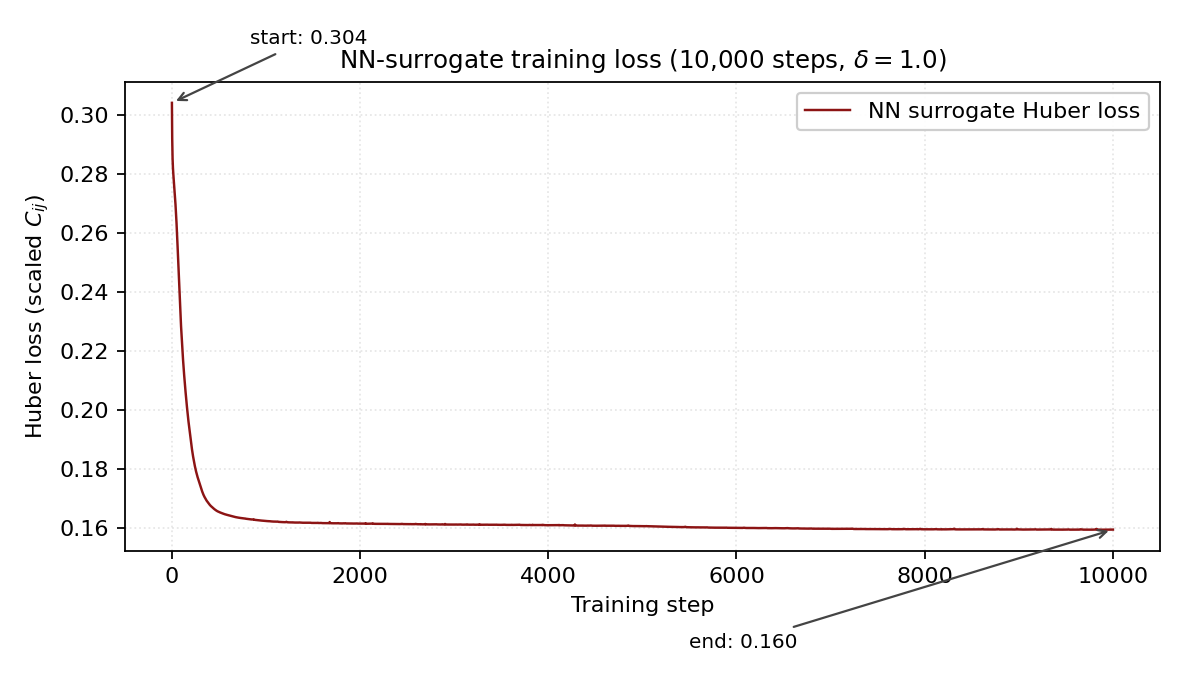
\includegraphics[width=0.96\linewidth]{figures/nnip_training_loss.png}\\[-0.4em]
\scriptsize Surrogate Huber-loss decay from $1.0$ to $0.16$ over
$10^{4}$ steps.

\column{0.52\textwidth}
\centering
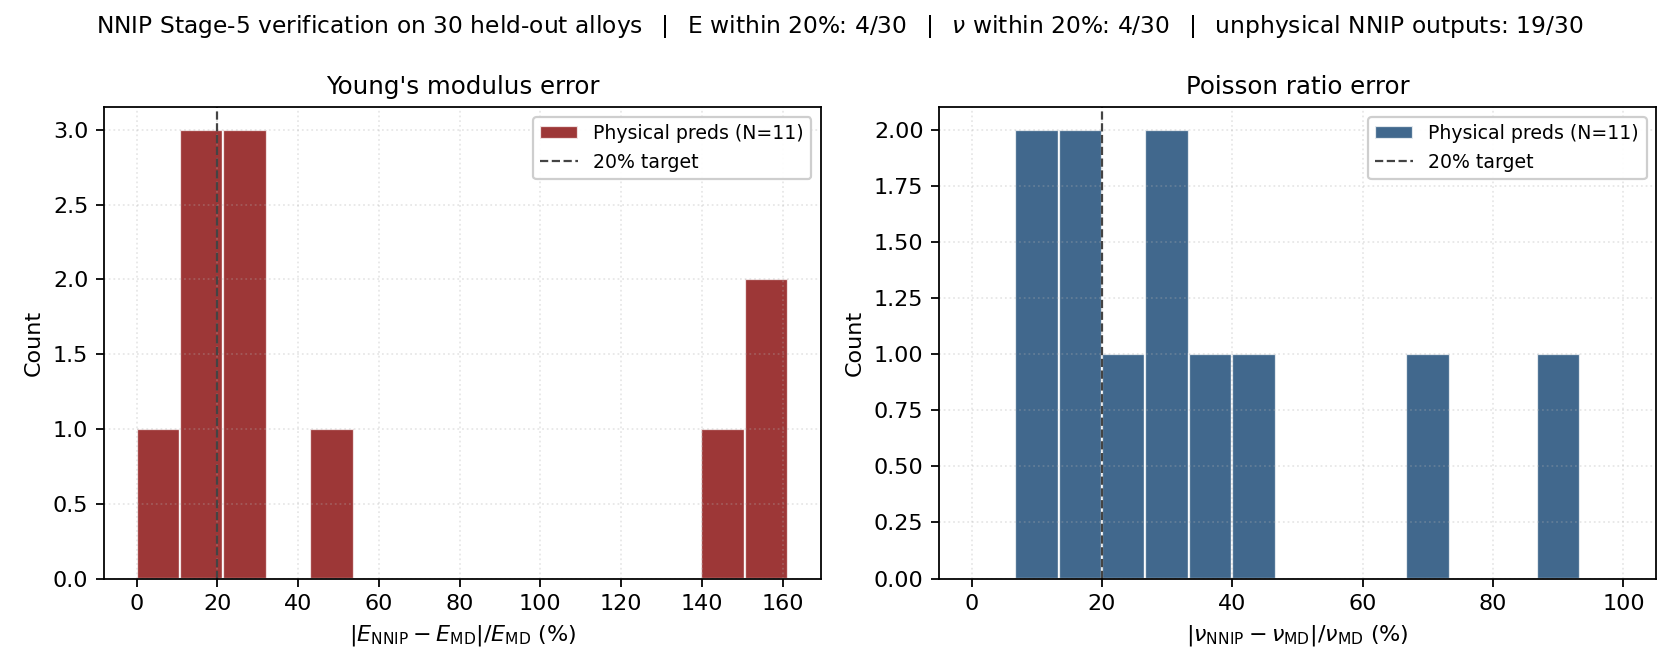
\includegraphics[width=0.96\linewidth]{figures/nnip_verification_errors.png}\\[-0.2em]

\scriptsize
\setlength{\tabcolsep}{3pt}
\renewcommand{\arraystretch}{0.88}
\begin{tabular}{lr}
\toprule
Held-out alloys / pass stability filter   & 30 / 11 \\
Within 20\,\% of MD on $E$ / on $\nu$       & 4 / 4 \\
Median error on $E$ / $\nu$ (physical)    & 23\,\% / 26\,\% \\
\bottomrule
\end{tabular}\\[0.25em]

\textbf{Verification outcome.}\\
\scriptsize Of the 30 held-out alloys, 19 violate the Born--Cauchy
stability criterion. Among the 11 stable predictions, 4 satisfy
the 20\,\% engineering tolerance on both $E$ and $\nu$.
\end{columns}
\end{frame}
